\clearpage
\newpage
\onecolumn
\begin{appendix}
\subsection{Implementation Details}
\ours mainly consists of two parts: perception and decision. We now detail the implementation details of each part as follows. The official implementation of DP3 is available on \url{https://github.com/YanjieZe/3D-Diffusion-Policy}.

\noindent\textbf{Perception.} The input of \ours includes the visual observation and the robot pose. The visual observation is a point cloud without colors, downsampled from the raw point cloud using Farthest Point Sampling (FPS). We use 512 or 1024 in all the simulated and real-world tasks. DP3 encodes the point cloud into a compact representation with our designed DP3 Encoder. We provide a simple PyTorch implementation of our DP3 Encoder as follows:
\begin{lstlisting}[language=Python, frame=none, basicstyle=\small\ttfamily, commentstyle=\color{ourblue}\small\ttfamily,columns=fullflexible, breaklines=true, postbreak=\mbox{\textcolor{red}{$\hookrightarrow$}\space}, escapeinside={(*}{*)}]
class DP3Encoder(nn.Module):
    def __init__(self, channels=3):
        # We only use xyz (channels=3) in this work
        # while our encoder also works for xyzrgb (channels=6) in our experiments
        self.mlp = nn.Sequential(
                nn.Linear(channels, 64), nn.LayerNorm(64), nn.ReLU(),
                nn.Linear(64, 128), nn.LayerNorm(128), nn.ReLU(),
                nn.Linear(128, 256), nn.LayerNorm(256), nn.ReLU())
        self.projection = nn.Sequential(nn.Linear(256, 64), nn.LayerNorm(64))
    
    def forward(self, x):
        # x: B, N, 3
        x = self.mlp(x) # B, N, 256
        x = torch.max(x, 1)[0] # B, 256
        x = self.projection(x) # B, 64
        return x
\end{lstlisting}
The robot poses are also processed by an MLP network described as follows:
\begin{lstlisting}[language=Python, frame=none, basicstyle=\small\ttfamily, commentstyle=\color{ourblue}\small\ttfamily,columns=fullflexible, breaklines=true, postbreak=\mbox{\textcolor{red}{$\hookrightarrow$}\space}, escapeinside={(*}{*)}]
# DimRobo is the dimension of the robot poses.
Sequential(
  (0): Linear(in_features=DimRobo, out_features=64, bias=True)
  (1): ReLU()
  (2): Linear(in_features=64, out_features=64, bias=True))
\end{lstlisting}
The representations encoded from point clouds and robot poses are concatenated into one representation of dimension 128.  Afterward, the decision backbone generates actions conditioning on this representation.

\noindent\textbf{Decision.} The decision backbone is a convolutional network-based diffusion policy, which transforms random Gaussian noise into a coherent sequence of actions. For implementation, we utilize the official PyTorch framework available from \citep{chi2023diffusion_policy}. In practice, the model is designed to predict a series of $H$ actions based on $N_{obs}$ observed timesteps, but it will only execute the last $N_{act}$ actions during inference. We set $H=4, N_{obs}=2, N_{act}=3$ for \ours and diffusion-based baselines.


The original Diffusion Policy typically employs a longer horizon, primarily due to the denser nature of the timesteps in their tasks.  In Table~\ref{table:prediction horizon}, we show that there is no significant difference between a short horizon and a long horizon for our tasks. Moreover, considering the potential for sudden disruptions in real-world robotic operations, we choose to employ a shorter horizon.

\noindent\textbf{Normalization.} We scale the min and max of each action dimension and each observation dimension to $[-1, 1]$ independently. Normalizing the actions to $[-1,1]$ is a must for the prediction of DDPM and DDIM since they would clip the prediction to $[-1,1]$ for stability. 

\subsection{Task Suite}

\noindent\textbf{Simulated tasks.} We collect diverse simulated tasks to systematically evaluate imitation learning algorithms. Our collected tasks mainly focus on robotic manipulation, including   Adroit~\citep{rajeswaran2017dapg}, Bi-DexHands~\citep{chen2022bidexhands}, DexArt~\citep{bao2023dexart}, DexDeform~\citep{li2023dexdeform}, DexMV~\citep{qin2022dexmv}, HORA~\citep{qi2023hora}, and MetaWorld~\citep{yu2020metaworld}. The full task names could be seen in Table~\ref{table: simulation results}. We add the support for 3D modality in these tasks when the 3D modality is not available originally. 

% \begin{table*}[t]
\centering
\caption{\textbf{Task suite of \ours.} }
\label{table:tasks}
 \begin{minipage}{.5\linewidth}
\begin{tabular}{lcccccc}
\toprule


 Task $\backslash$ Setting (3+2+4+6+1+6+2=24)  & \# Demo & \# Rob & \# Obj \\
 
\midrule

\textbf{Adroit}~\citep{rajeswaran2017dapg} (MuJoCo) & \\
    ~Hammer & 10 & 1 & 2\\
    ~Door & 10 & 1 & 1\\
    ~Pen & 10 & 1 & 1\\

\midrule    
    
\textbf{DexMV}~\citep{qin2022dexmv} (MuJoCo) & \\
    ~Pour & 10 & 1 & 2\\
    ~Place Inside & 10 & 1 & 2\\

\midrule

\textbf{DexArt}~\citep{bao2023dexart} (Sapien) & \\
    ~Laptop & 50 & 1 & 1\\
    ~Toilet & 50 & 1 & 1\\
    ~Faucet & 50 & 1 & 1\\
    ~Bucket & 50 & 1 & 1\\

\midrule

\textbf{DexDeform}~\citep{li2023dexdeform} (PlasticineLab)\\
~Rope & 10 & 2 & 2\\
~Bun & 10 & 2 & 1 \\
~Dumpling & 10 & 2 & 1\\
~Wrap & 10 & 1 & 2\\
~Flip & 10 & 1 & 1\\
~Folding (4 Directions) & 10$\times$4 & 1 & 1\\

\midrule



\textbf{HORA}~\citep{qi2023hora} (IsaacGym) \\
~In-hand Rotation& 50 & 1 & 1\\

% \midrule

% \textbf{Visual Dexterity}~\citep{chen2023visual_dex} (IsaacGym) \\
% ~In-hand Reorientation& 200 & 1 & 1\\
\midrule

% \textbf{DeXtreme}~\citep{handa2023dextreme} (IsaacGym) \\
% ~In-hand Orientation & try 100 & 1 & 1 \\
% \midrule


\textbf{Bi-DexHands}~\citep{chen2022bidexhands} (IsaacGym) \\

~Block Stack & 10 & 2 & 2\\
~Bottle Cap & 10 & 2 & 2 \\
% ~Door Close Inward & 10 & 2 & 2 \\
~Door Open Outward & 10 & 2 & 2 \\
~Grasp And Place & 10 & 2 & 2 \\
% ~Kettle & 10 & 2 & 2 \\
~Hand Over & 10 & 2 & 1 \\
~Scissors & 10 & 2 & 1 \\
% ~Catch Abreast & to try 100 (10:0)& 2& 1 \\
% ~Catch Over 2 Underarm & to try 100 (10: 0) & 2 & 1 \\
% ~Lift Underarm & to try 100 (10: 0) & 2 & 1 \\

% ~Pen &  & 2 & 2 \\
% \midrule
% \textbf{Eureka}~\citep{ma2023eureka} (IsaacGym) \\

% ~Spin & more than 1000 & 1 & 1 \\
% ~Spin Upside Down & more than 1000 & 1 & 1 \\

% \textbf{RoboMimic}~\citep{mandlekar2021robomimic} (MuJoCo)\\

% ~Lift & 10 & 1 & 1\\
% ~Square & 200 & 1 & 2\\

% ~Tool Hang & TBD \\
\midrule
\textbf{Real Robot}\\
~Dumpling  & \\
~Burrito & \\
~Drill & \\
~Scissors & \\
~In-hand Rotation~\citep{yuan2023robot_synthethesia} & \\
\bottomrule
\end{tabular}
 \end{minipage}
%  \begin{minipage}{.45\linewidth}
% \begin{tabular}{lcccccc}
% \toprule


%  Task $\backslash$ Setting (50) & \# Demo & \# Rob & \# Obj \\
 
% \midrule
% \textbf{MetaWorld}~\citep{yu2020metaworld} (MuJoCo) \\
% \textbf{Easy}\\
% ~Button Press & 10 & 1 & 1 \\
% ~Button Press Topdown & 10 & 1 & 1 \\
% ~Button Press Topdown Wall & 10 & 1 & 1 \\
% ~Button Press Wall & 10 & 1 & 1 \\
% ~Coffee Button & 10 & 1 & 2 \\
% ~Dial Turn & 10 & 1 & 1 \\
% ~Door Close & 10 & 1 & 1 \\
% ~Door Lock & 10 & 1 & 1 \\
% ~Door Open & 10 & 1 & 1 \\
% ~Door Unlock & 10 & 1 & 1 \\
% ~Drawer Close & 10 & 1 & 1 \\
% ~Drawer Open & 10 & 1 & 1 \\
% ~Faucet Close & 10 & 1 & 1 \\
% ~Faucet Open & 10 & 1 & 1 \\
% ~Handle Press & 10 & 1 & 1 \\
% ~Handle Press Side & 10 & 1 & 1 \\
% ~Handle Pull & 10 & 1 & 1 \\
% ~Handle Pull Side & 10 & 1 & 1 \\
% ~Lever Pull & 10 & 1 & 1 \\
% ~Plate Slide & 10 & 1 & 1 \\
% ~Plate Slide Back & 10 & 1 & 1 \\
% ~Plate Slide Back Side & 10 & 1 & 1 \\
% ~Plate Slide Side & 10 & 1 & 1 \\
% ~Reach & 10 & 1 & 1 \\
% ~Reach Wall & 10 & 1 & 1 \\
% ~Window Close & 10 & 1 & 1 \\
% ~Window Open & 10 & 1 & 1 \\
% ~Peg Unplug Side & 10 & 1 & 1 \\
% \textbf{Medium}\\
% ~Basketball & 10 & 1 & 2 \\
% ~Bin Picking & 10 & 1 & 2 \\
% ~Box Close & 10 & 1 & 2 \\
% ~Coffee Pull & 10 & 1 & 2 \\
% ~Coffee Push & 10 & 1 & 2 \\
% ~Hammer & 10 & 1 & 2 \\
% ~Peg Insert Side & 10 & 1 & 2 \\
% ~Push Wall & 10 & 1 & 2 \\
% ~Soccer & 10 & 1 & 2 \\
% ~Sweep & 10 & 1 & 1 \\
% ~Sweep Into & 10 & 1 & 1 \\
% \textbf{Hard}\\
% ~Assembly & 10 & 1 & 2 \\
% ~Hand Insert & 10 & 1 & 1 \\
% ~Pick Out of Hole & 10 & 1 & 1 \\
% ~Pick Place & 10 & 1 & 1 \\
% ~Push & 10 & 1 & 1 \\
% ~Push Back & 10 & 1 & 1 \\
% \textbf{Very Hard}\\
% ~Shelf Place & 10 & 1 & 2 \\
% ~Disassemble & 10 & 1 & 2 \\
% ~Stick Pull & 10 & 1 & 1 \\
% ~Stick Push & 10 & 1 & 1 \\
% ~Pick Place Wall & 10  & 1 & 2 \\

% % \midrule
% % \textbf{MetaWorld}~\citep{yu2020metaworld} (MuJoCo) \\
% % \textbf{Easy}\\
% % ~Button Press & 10 & 1 & ? \\
% % ~Button Press Topdown & 10 & 1 & ? \\
% % ~Button Press Topdown Wall & 10 & 1 & ? \\
% % ~Button Press Wall & 10 & 1 & ? \\
% % ~Coffee Button & 10 & 1 & ? \\
% % ~Dial Turn & 10 & 1 & ? \\
% % ~Door Close & 10 & 1 & ? \\
% % ~Door Lock & 10 & 1 & ? \\
% % ~Door Open & 10 & 1 & ? \\
% % ~Door Unlock & 10 & 1 & ? \\
% % ~Drawer Close & 10 & 1 & ? \\
% % ~Drawer Open & 10 & 1 & ? \\
% % ~Faucet Close & 10 & 1 & ? \\
% % ~Faucet Open & 10 & 1 & ? \\
% % ~Handle Press & 10 & 1 & ? \\
% % ~Handle Press Side & 10 & 1 & ? \\
% % ~Handle Pull & 10 & 1 & ? \\
% % ~Handle Pull Side & 10 & 1 & ? \\
% % ~Lever Pull & 10 & 1 & ? \\
% % ~Plate Slide & 10 & 1 & ? \\
% % ~Plate Slide Back & 10 & 1 & ? \\
% % ~Plate Slide Back Side & 10 & 1 & ? \\
% % ~Plate Slide Side & 10 & 1 & ? \\
% % ~Reach & 10 & 1 & ? \\
% % ~Reach Wall & 10 & 1 & ? \\
% % ~Window Close & 10 & 1 & ? \\
% % ~Window Open & 10 & 1 & ? \\
% % ~Peg Unplug Side & 10 & 1 & ? \\
% % \textbf{Medium}\\
% % ~Basketball & 10 & 1 & ? \\
% % ~Bin Picking & fail & 1 & ? \\
% % ~Box Close & 20 & 1 & ? \\
% % ~Coffee Pull & 10 & 1 & ? \\
% % ~Coffee Push & 10 & 1 & ? \\
% % ~Hammer & 200 & 1 & ? \\
% % ~Peg Insert Side & 20 & 1 & ? \\
% % ~Push Wall & 200 & 1 & ? \\
% % ~Soccer & 300 & 1 & ? \\
% % ~Sweep & 10 & 1 & ? \\
% % ~Sweep Into & 100 & 1 & ? \\
% % \textbf{Hard}\\
% % ~Assembly & 10 & 1 & ? \\
% % ~Hand Insert & fail & 1 & ? \\
% % ~Pick Out of Hole & ? & 1 & ? \\
% % ~Pick Place & 100 & 1 & ? \\
% % ~Push & 100 & 1 & ? \\
% % ~Push Back & 100 & 1 & ? \\
% % \textbf{Very Hard}\\
% % ~Shelf Place & 100 & 1 & ? \\
% % ~Disassemble & 200 & 1 & ? \\
% % ~Stick Pull & 20 & 1 & ? \\
% % ~Stick Push & 10 & 1 & ? \\
% % ~Pick Place Wall & 300  & 1 & ? \\

% \bottomrule
% \end{tabular}
%   \end{minipage}
\end{table*}





\noindent\textbf{Real-world tasks.} The episode length for our real-world tasks is not fixed. Average episode lengths for demonstrations of each task are listed as follows: (1) 79.9 for Roll-Up; (2) 113.5 for Dumpling; (3) 71.4 for Drill; and (4) 83.6 for Pour. During the evaluation of the policy, we stop the robot when we find (1) the policy finishes the task; (2) the policy can not successfully handle the task; and (3) the policy makes behaviors that are harmful to the hardware. Our real-world setup and everyday objects used in our tasks are shown in Figure~\ref{fig:real world setup}. The randomization in each task is shown in Figure~\ref{fig:real task randomness}. For Roll-Up and Dumpling, the plasticine's shape and the appearance of the objects placed upon the plasticine are randomized. For Drill and Pour, the variations come from the random positions of the cube, drill, and bowl. 



\subsection{More Simulation Experiments}
\label{appendix: full simulation results}

\noindent\textbf{Simulation results for each task.} We give the simulation results for each task in Table~\ref{table: simulation results}, which is supplementary to Table~\ref{table:simulation simplified} in our main paper. We report average success rates across 3 seeds. For HORA,  we report the normalized returns since this task is doing in-hand rotation and is not measured by success rates.



\noindent\textbf{Success rates for experts.} In our simulated tasks, we apply Reinforcement Learning (RL)-trained agents to generate demonstrations. These expert policies are rigorously evaluated over 200 episodes, and their success rates are detailed in Table~\ref{table: expert SR}. For MetaWorld tasks, we present results from scripted policies.







 

\noindent\textbf{Choice of prediction horizon.} DP3 applies a short action prediction and execution horizon $H=4, N_{act}=3$, and so does the baseline Diffusion Policy. This is mainly designed for the generality of \ours in complex tasks and real robot tasks, where the environment would be changed by human intervention and the policy needs to switch action immediately. As shown in Table~\ref{table:prediction horizon}, a shortened prediction horizon is competitive with a longer one.

\begin{table}[htbp]
\centering
\vspace{-0.1in}
\caption{\textbf{Ablation on prediction horizon.} In this work, \ours and Diffusion Policy uses a prediction horizon $H=4, N_{act}=3$. We test $H=16, N_{act}=8$ originally used in \citep{chi2023diffusion_policy} for both methods.}
\label{table:prediction horizon}
\vspace{-0.05in}
\resizebox{0.65\textwidth}{!}{
\begin{tabular}{l|cccccc|ccc}
\toprule

  Algorithm & H & D  & P & A & DA & SP & \textbf{Average} \\

\midrule


\ours & \dd{100}{0} & \dd{62}{4} & \dd{43}{6} & \dd{99}{1} & \dd{69}{4} & \dd{97}{4} & $78.3$\\

w/ long horizon & \dd{100}{0} & \dd{64}{5} & \dd{46}{3} & \dd{99}{1} & \dd{75}{3} & \dd{85}{14} & $78.2$ \\
 
 \midrule
 
Diffusion Policy &	\dd{48}{17} & \dd{50}{5} & \dd{25}{4}	& \dd{15}{1} & \dd{43}{7} & 	\dd{63}{3} & $40.7$\\

w/ long horizon & \dd{68}{11} & \dd{44}{4} & \dd{16}{2} & \dd{12}{3} & \dd{14}{1} & \dd{44}{5} & $33.0$ \\


\bottomrule
\end{tabular}}
\end{table}







\subsection{Simple DP3}

\begin{wrapfigure}{r}{0.35\textwidth}
\vspace{-0.35in}
    \centering
     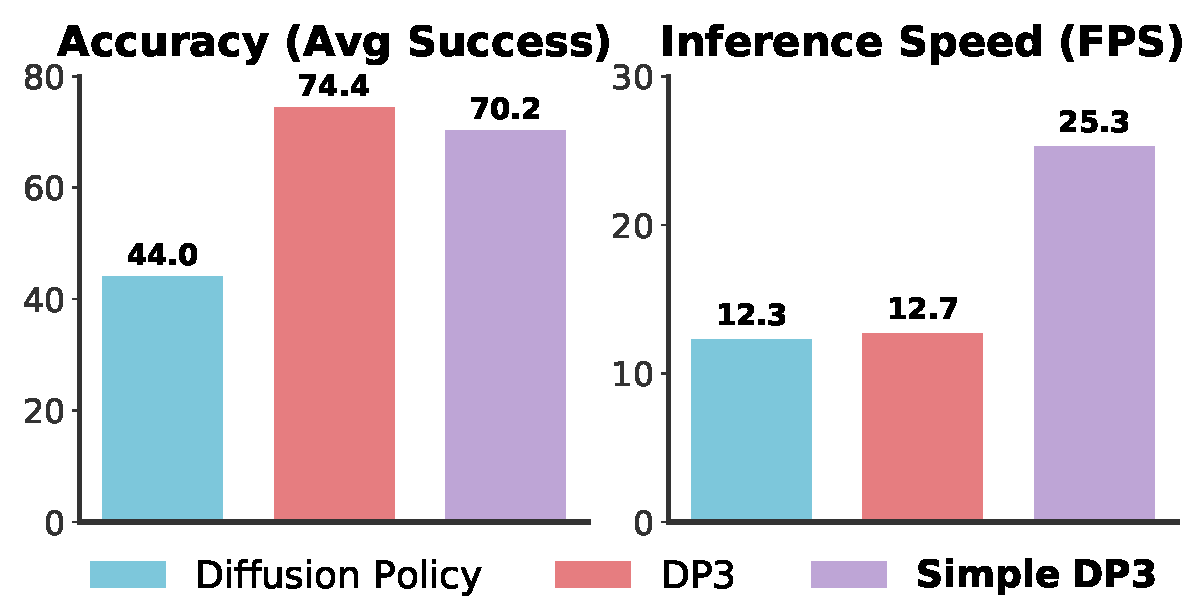
\includegraphics[width=0.35\textwidth]{figures/simple_DP3.pdf}
    % \vspace{-0.2in}
\end{wrapfigure}

To enhance the applicability of DP3 in real-world robot learning, we simplify the policy backbone of DP3, which is identified as one critical factor that impacts inference speed. The refined version, dubbed \textbf{\textit{Simple DP3}}, offers 2x inference speed while maintaining high accuracy, as shown in Table~\ref{tab:summary simple DP3}. The efficiency stems from removing the redundant components in the UNet backbone. The implementation of Simple DP3 is available on \url{https://github.com/YanjieZe/3D-Diffusion-Policy}.



\begin{table}[htbp]
    \centering
    % \vspace{-0.1in}
     \caption{\textbf{Results of Simple DP3.} Compared to DP3, Simple DP3 achieves nearly 2x inference speed without losing much accuracy. Full evaluation results are given in Table~\ref{table: simple DP3}.}
    \label{tab:summary simple DP3}
    \vspace{-0.05in}
    \begin{tabular}{l|ccc}
    \toprule
         Algorithm & Diffusion Policy & DP3  & \textbf{Simple DP3} \\
         \midrule
        Inference Speed (FPS) & $12.3$ & $12.7$ & $25.3$ ($\uparrow \mathbf{99}\%$) \\
        Accuracy (Avg Success) & $44.0$ &  $74.4$ & $70.2$ ($\downarrow \mathbf{6}\%$) \\
        \bottomrule
    \end{tabular}

\end{table}

\begin{table*}[htbp]
\centering
\vspace{-0.2in}
\caption{\textbf{Full evaluation results of Simple DP3.} We evaluate Simple DP3 on 10 tasks and compare it with DP3 and find that Simple DP3 could achieve results very competitive to DP3.}
\vspace{-0.05in}
\label{table: simple DP3}
\resizebox{0.9\textwidth}{!}{%
\begin{tabular}{l|ccc|ccc|cccc|cc}
\toprule

% & \multicolumn{3}{c}{\textbf{Adroit}} & \multicolumn{3}{c}{\textbf{MetaWorld}} \\
 % Algorithm & Hammer & Door  & Pen & Assembly & Basketball & Shelf Place & \textbf{Average} \\
    & \multicolumn{3}{c|}{Adroit} & \multicolumn{3}{c|}{MetaWorld} & \multicolumn{4}{c|}{DexArt} & \\
  Algorithm $\backslash$  Task & Hammer & Door  & Pen & Assembly & Disassemble & Stick-Push & Laptop & Faucet & Toilet & Bucket & \textbf{Average} \\


\midrule


\textbf{\ours} & \ddbf{100}{0} & \ddbf{62}{4} & \ddbf{43}{6} & \ddbf{99}{1} & \ddbf{69}{4} & \ddbf{97}{4} & \ddbf{83}{1} & \ddbf{63}{2} & \ddbf{82}{4} & \ddbf{46}{2} & \ccbf{74.4}\\

Diffusion Policy &	\dd{48}{17} & \dd{50}{5} & \dd{25}{4}	& \dd{15}{1} & \dd{43}{7} & 	\dd{63}{3} & \dd{69}{4} & \dd{23}{8}  & \dd{58}{2} & \ddbf{46}{1} & $44.0$ \\


\textbf{Simple DP3} & \ddbf{100}{0} & \dd{58}{4} & \ddbf{46}{5} & \dd{79}{1} & \dd{50}{3} & \ddbf{97}{5} & \ddbf{84}{2} & \ddbf{63}{3} & \dd{81}{6} & \dd{44}{6} & $70.2$ \\


\bottomrule
\end{tabular}}
\vspace{-0.2in}
\end{table*}



\begin{table*}[htbp]
\centering
\caption{\textbf{Main results on 72 simulation tasks.} Results for each task are provided in this table. A summary across domains is shown in Table~\ref{table:simulation simplified}. }
\label{table: simulation results}
\begin{flushleft}
\resizebox{0.9\textwidth}{!}{%
\begin{tabular}{l|ccc|ccccccc}
\toprule
& \multicolumn{3}{c|}{\textbf{Adroit}~\citep{rajeswaran2017dapg}} & \multicolumn{6}{c}{\textbf{Bi-DexHands}~\citep{chen2022bidexhands}} \\

 Alg $\backslash$ Task & Hammer  & Door & Pen & Block Stack & Bottle Cap & Door Open Outward & Grasp And Place & Hand Over & Scissors\\
 
\midrule

 
\ours &  \ddbf{100}{0} & \ddbf{62}{4} & \ddbf{43}{6} & \ddbf{24}{15} & \ddbf{83}{10} & \ddbf{100}{0} & \ddbf{69}{22} & \ddbf{45}{8} & \ddbf{100}{0} \\
 Diffusion Policy &   \dd{45}{5} & \dd{37}{2} & \dd{13}{2} & \dd{4}{4} & \dd{61}{5}  & \ddbf{100}{0} & \dd{65}{9} & \dd{38}{0} & \ddbf{100}{0} \\
\bottomrule
\end{tabular}}

\resizebox{0.9\textwidth}{!}{%
\begin{tabular}{l|cccc|cccccc|cc|cc}
\toprule
& \multicolumn{4}{c|}{\textbf{DexArt}~\citep{bao2023dexart}} & \multicolumn{6}{c|}{\textbf{DexDeform}~\citep{li2023dexdeform}} & \multicolumn{2}{c|}{\textbf{DexMV}~\citep{qin2022dexmv}} & \textbf{HORA}~\citep{qi2023hora}\\

 Alg $\backslash$ Task & Laptop & Faucet & Toilet & Bucket & Rope & Bun & Dumpling & Wrap & Flip & Folding & Pour & Place Inside & Rotation\\
 
\midrule

\ours & \ddbf{83}{1}  & \ddbf{63}{2} & \ddbf{82}{4} & \ddbf{46}{2} & \dd{93}{2} & \dd{70}{9} & \ddbf{92}{0} & \ddbf{94}{0} & \dd{97}{1} &  \dd{81}{2} & \ddbf{99}{2} & \ddbf{100}{0}  & \ddbf{71}{31}   \\

 Diffusion Policy & \dd{69}{4} & \dd{23}{8} & \dd{58}{2} & \ddbf{46}{1} & \ddbf{97}{0} & \ddbf{76}{4} &  \ddbf{92}{0} & \dd{91}{0} & \ddbf{99}{0} & \ddbf{88}{1} & \dd{90}{2} & \ddbf{100}{0} & \dd{49}{11} \\
\bottomrule
\end{tabular}}



\resizebox{0.9\textwidth}{!}{%
\begin{tabular}{l|cccccccc}
\toprule
& \multicolumn{7}{c}{\textbf{Meta-World~\citep{yu2020metaworld} (Easy)}} \\

 Alg $\backslash$ Task & Button Press & Button Press Topdown & Button Press Topdown Wall & Button Press Wall & Coffee Button & Dial Turn & Door Close \\
\midrule

\ours & \ddbf{100}{0} & \ddbf{100}{0} & \ddbf{99}{2} & \ddbf{99}{1} & \ddbf{100}{0} & \ddbf{66}{1} &  \ddbf{100}{0}     \\
 Diffusion Policy & \dd{99}{1} & \dd{98}{1} & \dd{96}{3} & \dd{97}{3} & \dd{99}{1} & \dd{63}{10} & \ddbf{100}{0}  \\

\bottomrule
\end{tabular}}



\resizebox{0.9\textwidth}{!}{%
\begin{tabular}{l|ccccccccccc}
\toprule
& \multicolumn{9}{c}{\textbf{Meta-World (Easy)}} \\

 Alg $\backslash$ Task & Door Lock & Door Open & Door Unlock & Drawer Close & Drawer Open & Faucet Close & Faucet Open & Handle Press & Handle Pull\\
\midrule
\ours & \ddbf{98}{2} & \ddbf{99}{1} & \ddbf{100}{0} &   \ddbf{100}{0} & \ddbf{100}{0} & \ddbf{100}{0} & \ddbf{100}{0} & \ddbf{100}{0} &  \ddbf{53}{11} &     \\
 Diffusion Policy &  \dd{86}{8} & \dd{98}{3}& \dd{98}{3}& \ddbf{100}{0}& \dd{93}{3}& \ddbf{100}{0}& \ddbf{100}{0}& \dd{81}{4}& \dd{27}{22} \\

\bottomrule
\end{tabular}}


\resizebox{0.9\textwidth}{!}{%
\begin{tabular}{l|ccccccccccc}
\toprule
& \multicolumn{8}{c}{\textbf{Meta-World (Easy)}} \\

 Alg $\backslash$ Task & Handle Press Side & Handle Pull Side & Lever Pull & Plate Slide & Plate Slide Back & Plate Slide Back Side & Plate Slide Side & Reach\\
\midrule

\ours & \ddbf{100}{0} & \ddbf{85}{3} & \ddbf{79}{8} & \ddbf{100}{1} & \ddbf{99}{0} & \ddbf{100}{0} & \ddbf{100}{0} & \ddbf{24}{1}\\

Diffusion Policy & \ddbf{100}{0}& \dd{23}{17}& \dd{	49}{5}& \dd{	83}{4}& \ddbf{	99}{0}& \ddbf{	100}{0}& \ddbf{	100}{0}& \dd{	18}{2}\\

\bottomrule
\end{tabular}}




\resizebox{0.9\textwidth}{!}{%
\begin{tabular}{l|cccc|ccccccc}
\toprule
& \multicolumn{4}{c|}{\textbf{Meta-World (Easy)}} & \multicolumn{5}{c}{\textbf{Meta-World (Medium)}} \\

 Alg $\backslash$ Task & Reach Wall & Window Close & Window Open & Peg Unplug Side & Basketball & Bin Picking & Box Close & Coffee Pull & Coffee Push\\
\midrule

\ours & \ddbf{68}{3}& \ddbf{100}{0}& \ddbf{100}{0}& \ddbf{75}{5} & \ddbf{98}{2} & \ddbf{34}{30} & \ddbf{42}{3} & \ddbf{87}{3} & \ddbf{94}{3}\\
 Diffusion Policy &\dd{59}{7}&\dd{100}{0}&\dd{100}{0}&\dd{74}{3} &\dd{85}{6}&\dd{15}{4}&\dd{30}{5}&\dd{34}{7}&\dd{67}{4} \\

\bottomrule
\end{tabular}}






\resizebox{0.9\textwidth}{!}{%
\begin{tabular}{l|cccccc|ccccc}
\toprule
& \multicolumn{6}{c|}{\textbf{Meta-World (Medium)}} & \multicolumn{4}{c}{\textbf{Meta-World (Hard)}} \\

 Alg $\backslash$ Task & Hammer & Peg Insert Side & Push Wall & Soccer & Sweep & Sweep Into & Assembly & Hand Insert & Pick Out of Hole & Pick Place\\
\midrule

\ours & \ddbf{76}{4}& \ddbf{69}{7}& \ddbf{49}{8}& \ddbf{18}{3}& \ddbf{96}{3}& \ddbf{15}{5}& \ddbf{99}{1}& \ddbf{14}{4}& \ddbf{14}{9}& \ddbf{12}{4}\\

 Diffusion Policy & \dd{15}{6}& \dd{34}{7}& \dd{20}{3}& \dd{14}{4}& \dd{18}{8}& \dd{10}{4}& \dd{15}{1}& \dd{9}{2}& \dd{0}{0}& \dd{0}{0}\\




\bottomrule
\end{tabular}}


\resizebox{0.9\textwidth}{!}{%
\begin{tabular}{l|cc|ccccc|ccccccc}
\toprule
& \multicolumn{2}{c|}{\textbf{Meta-World (Hard)}} & \multicolumn{5}{c|}{\textbf{Meta-World (Very Hard)}} & 
 \multicolumn{1}{c}{\multirow{2}{*}{\textbf{Average}}} & \\

 Alg $\backslash$ Task & Push & Push Back & Shelf Place & Disassemble & Stick Pull & Stick Push & Pick Place Wall &  \\
\midrule

\ours & \ddbf{51}{3}& \ddbf{0}{0}& \ddbf{17}{10}& \ddbf{69}{4}& \ddbf{27}{8}& \ddbf{97}{4}& \ddbf{35}{8} &  \multicolumn{1}{c}{\ccbf{74.4}}\\

 Diffusion Policy &\dd{30}{3}& \dd{0}{0}& \dd{11}{3}& \dd{43}{7}& \dd{11}{2}& \dd{63}{3}& \dd{5}{1} & \multicolumn{1}{c}{{59.8}}\\

\bottomrule
\end{tabular}}


\end{flushleft}
\end{table*}






\begin{table*}[htbp]
\centering
\caption{\textbf{Success rates of experts on 72 simulation tasks.} We evaluate 200 episodes for each task. For MetaWorld tasks, we evaluate both BAC agents and the script policies provided officially in MetaWorld. For DexDeform tasks, the demonstrations are collected by human teleportation~\citep{li2023dexdeform} and we record the success rates as 100\%.}
\label{table: expert SR}
\vspace{-0.1in}
\begin{flushleft}
\resizebox{0.9\textwidth}{!}{%
\begin{tabular}{l|ccc|ccccccc}
\toprule
& \multicolumn{3}{c|}{\textbf{Adroit}~\citep{rajeswaran2017dapg}} & \multicolumn{6}{c}{\textbf{Bi-DexHands}~\citep{chen2022bidexhands}} \\

 Alg $\backslash$ Task & Hammer  & Door & Pen & Block Stack & Bottle Cap & Door Open Outward & Grasp And Place & Hand Over & Scissors\\
 
\midrule

Expert & \cc{99.0} & \cc{100.0} & \cc{97.0} & \cc{83.5} & \cc{100.0} & \cc{100.0} & \cc{100.0} & \cc{77.0} & \cc{99.5}\\
 
\bottomrule
\end{tabular}}

\resizebox{0.9\textwidth}{!}{%
\begin{tabular}{l|cccc|cccccc|cc|cc}
\toprule
& \multicolumn{4}{c|}{\textbf{DexArt}~\citep{bao2023dexart}} & \multicolumn{6}{c|}{\textbf{DexDeform}~\citep{li2023dexdeform}} & \multicolumn{2}{c|}{\textbf{DexMV}~\citep{qin2022dexmv}} & \textbf{HORA}~\citep{qi2023hora}\\

 Alg $\backslash$ Task & Laptop & Faucet & Toilet & Bucket & Rope & Bun & Dumpling & Wrap & Flip & Folding & Pour & Place Inside & Rotation\\
 
\midrule

Expert & \cc{86.5} & \cc{58.0} & \cc{66.5} & \cc{80.0} & \cc{100.0} & \cc{100.0} &  \cc{100.0} & \cc{100.0} & \cc{100.0} & \cc{100.0} & \cc{88.5} & \cc{64.5} & \cc{80.5}\\
\bottomrule
\end{tabular}}



\resizebox{0.9\textwidth}{!}{%
\begin{tabular}{l|cccccccc}
\toprule
& \multicolumn{7}{c}{\textbf{Meta-World~\citep{yu2020metaworld} (Easy)}} \\

 Alg $\backslash$ Task & Button Press & Button Press Topdown & Button Press Topdown Wall & Button Press Wall & Coffee Button & Dial Turn & Door Close \\
\midrule

Expert & \cc{100.0} & \cc{100.0} & \cc{100.0} & \cc{98.5} & \cc{100.0} & \cc{100.0} & \cc{100.0}\\

\bottomrule
\end{tabular}}



\resizebox{0.9\textwidth}{!}{%
\begin{tabular}{l|ccccccccccc}
\toprule
& \multicolumn{9}{c}{\textbf{Meta-World (Easy)}} \\

 Alg $\backslash$ Task & Door Lock & Door Open & Door Unlock & Drawer Close & Drawer Open & Faucet Close & Faucet Open & Handle Press & Handle Pull\\
\midrule



 Expert & \cc{100.0} & \cc{98.5} & \cc{100.0} & \cc{100.0} &\cc{100.0} & \cc{100.0} & \cc{100.0} & \cc{100.0} & \cc{100.0}\\
 
\bottomrule
\end{tabular}}


\resizebox{0.9\textwidth}{!}{%
\begin{tabular}{l|ccccccccccc}
\toprule
& \multicolumn{8}{c}{\textbf{Meta-World (Easy)}} \\

 Alg $\backslash$ Task & Handle Press Side & Handle Pull Side & Lever Pull & Plate Slide & Plate Slide Back & Plate Slide Back Side & Plate Slide Side & Reach\\
\midrule

Expert & \cc{100.0} & \cc{100.0} & \cc{98.5} & \cc{100.0} & \cc{100.0} & \cc{100.0} & \cc{100.0} & \cc{100.0}\\
\bottomrule
\end{tabular}}




\resizebox{0.9\textwidth}{!}{%
\begin{tabular}{l|cccc|ccccccc}
\toprule
& \multicolumn{4}{c|}{\textbf{Meta-World (Easy)}} & \multicolumn{5}{c}{\textbf{Meta-World (Medium)}} \\

 Alg $\backslash$ Task & Reach Wall & Window Close & Window Open & Peg Unplug Side & Basketball & Bin Picking & Box Close & Coffee Pull & Coffee Push\\
\midrule


 Expert & \cc{100.0} & \cc{100.0} & \cc{100.0} & \cc{99.0} &\cc{100.0} & \cc{97.0} & \cc{90.0} & \cc{100.0} & \cc{100.0}\\
\bottomrule
\end{tabular}}






\resizebox{0.9\textwidth}{!}{%
\begin{tabular}{l|cccccc|ccccc}
\toprule
& \multicolumn{6}{c|}{\textbf{Meta-World (Medium)}} & \multicolumn{4}{c}{\textbf{Meta-World (Hard)}} \\

 Alg $\backslash$ Task & Hammer & Peg Insert Side & Push Wall & Soccer & Sweep & Sweep Into & Assembly & Hand Insert & Pick Out of Hole & Pick Place\\
\midrule



Expert & \cc{100.0} & \cc{92.0} & \cc{100.0} & \cc{90.5} &\cc{100.0} & \cc{90.0} & \cc{100.0} & \cc{100.0} & \cc{100.0} & \cc{100.0}\\
\bottomrule
\end{tabular}}

\resizebox{0.7\textwidth}{!}{%
\begin{tabular}{l|cc|cccccccccccc}
\toprule
& \multicolumn{2}{c|}{\textbf{Meta-World (Hard)}} & \multicolumn{5}{c}{\textbf{Meta-World (Very Hard)}}  


 % \multicolumn{2}{c}{\multirow{2}{*}{\textbf{Average}}}
  \\

 Alg $\backslash$ Task & Push & Push Back & Shelf Place & Disassemble & Stick Pull & Stick Push & Pick Place Wall  \\
\midrule


 Expert & \cc{100.0} & \cc{0.0} & \cc{99.5} & \cc{92.5} & \cc{95.0} & \cc{100.0} & \cc{99.5}\\
\bottomrule
\end{tabular}}
\end{flushleft}


\end{table*}








\end{appendix}


